\documentclass[%
 reprint,
%superscriptaddress,
%groupedaddress,
%unsortedaddress,
%runinaddress,
%frontmatterverbose, 
% preprint,
%preprintnumbers,
%nofootinbib,
%nobibnotes,
%bibnotes,
amsmath,amssymb,
aps,
onecolumn,
% pra,
%prb,
%rmp,
%prstab,
%prstper,
%floatfix,
]{revtex4-2}

\usepackage[dvipsnames]{xcolor}
\usepackage{braket}
\usepackage{caption}
\usepackage{subcaption}
\usepackage{graphicx}% Include figure files
\usepackage{dcolumn}% Align table columns on decimal point
\usepackage{bm}% bold math
%\usepackage{hyperref}% add hypertext capabilities
%\usepackage[mathlines]{lineno}% Enable numbering of text and display math
%\linenumbers\relax % Commence numbering lines

%\usepackage[showframe,%Uncomment any one of the following lines to test 
%%scale=0.7, marginratio={1:1, 2:3}, ignoreall,% default settings
%%text={7in,10in},centering,
%%margin=1.5in,
%%total={6.5in,8.75in}, top=1.2in, left=0.9in, includefoot,
%%height=10in,a5paper,hmargin={3cm,0.8in},
%]{geometry}

\begin{document}

\preprint{APS/123-QED}

\title{Tensor Network Methods in Quantum Error Correction}% Force line breaks with \\
% \thanks{A footnote to the article title}%

\author{Varun Seshadri }

\date{\today}

\begin{abstract}
    This is a short review on the different tensor network methods used in Quantum Error Correction.
    This was done while trying to resolve the dimension incompatibility issue in [FP2014]. Let's see what this leads to

\end{abstract}

%\keywords{Suggested keywords}%Use showkeys class option if keyword
%display desired
\maketitle

\section{MPS/MPO representations of topological codes}
\begin{itemize}
    \item BSV 14
    \item CF 12
    \item Chubb 2021
\end{itemize}


\section{PEPS representations of the topological codes}
\begin{itemize}
    \item DP 2017 for the surface codes.
    \item There was some other paper that used a PEPO representation, but I am unable to find it.
\end{itemize}

\section{Channel State Represenation}
\begin{itemize}
    \item FP 2014
    \item DP 2017
\end{itemize}

\section{Seed codes to construct QEC Codes}
\begin{itemize}
    \item The whole 9 yards from Terry Farrelly,
    \item Quantum Lego from Cao Lackey
    \item The whole shenanigans of Holographic codes
\end{itemize}


\section{On Stabilizer Channels}
Ferris in a talk titled, "Tensor Networks and Coding Theory", posits a channel picture for the decoding problem, wherein he introduces, stabilizer channels. The figure below illustrates his thoughts. Alex M-Hermes comments that this notation is misleading. I concur with this argument, especially w.r.t to the way, this notation was used in a paper in Quatum Thermodynamics paper titled Stabilizer channels. 

\begin{figure}[ht]
    \centering
    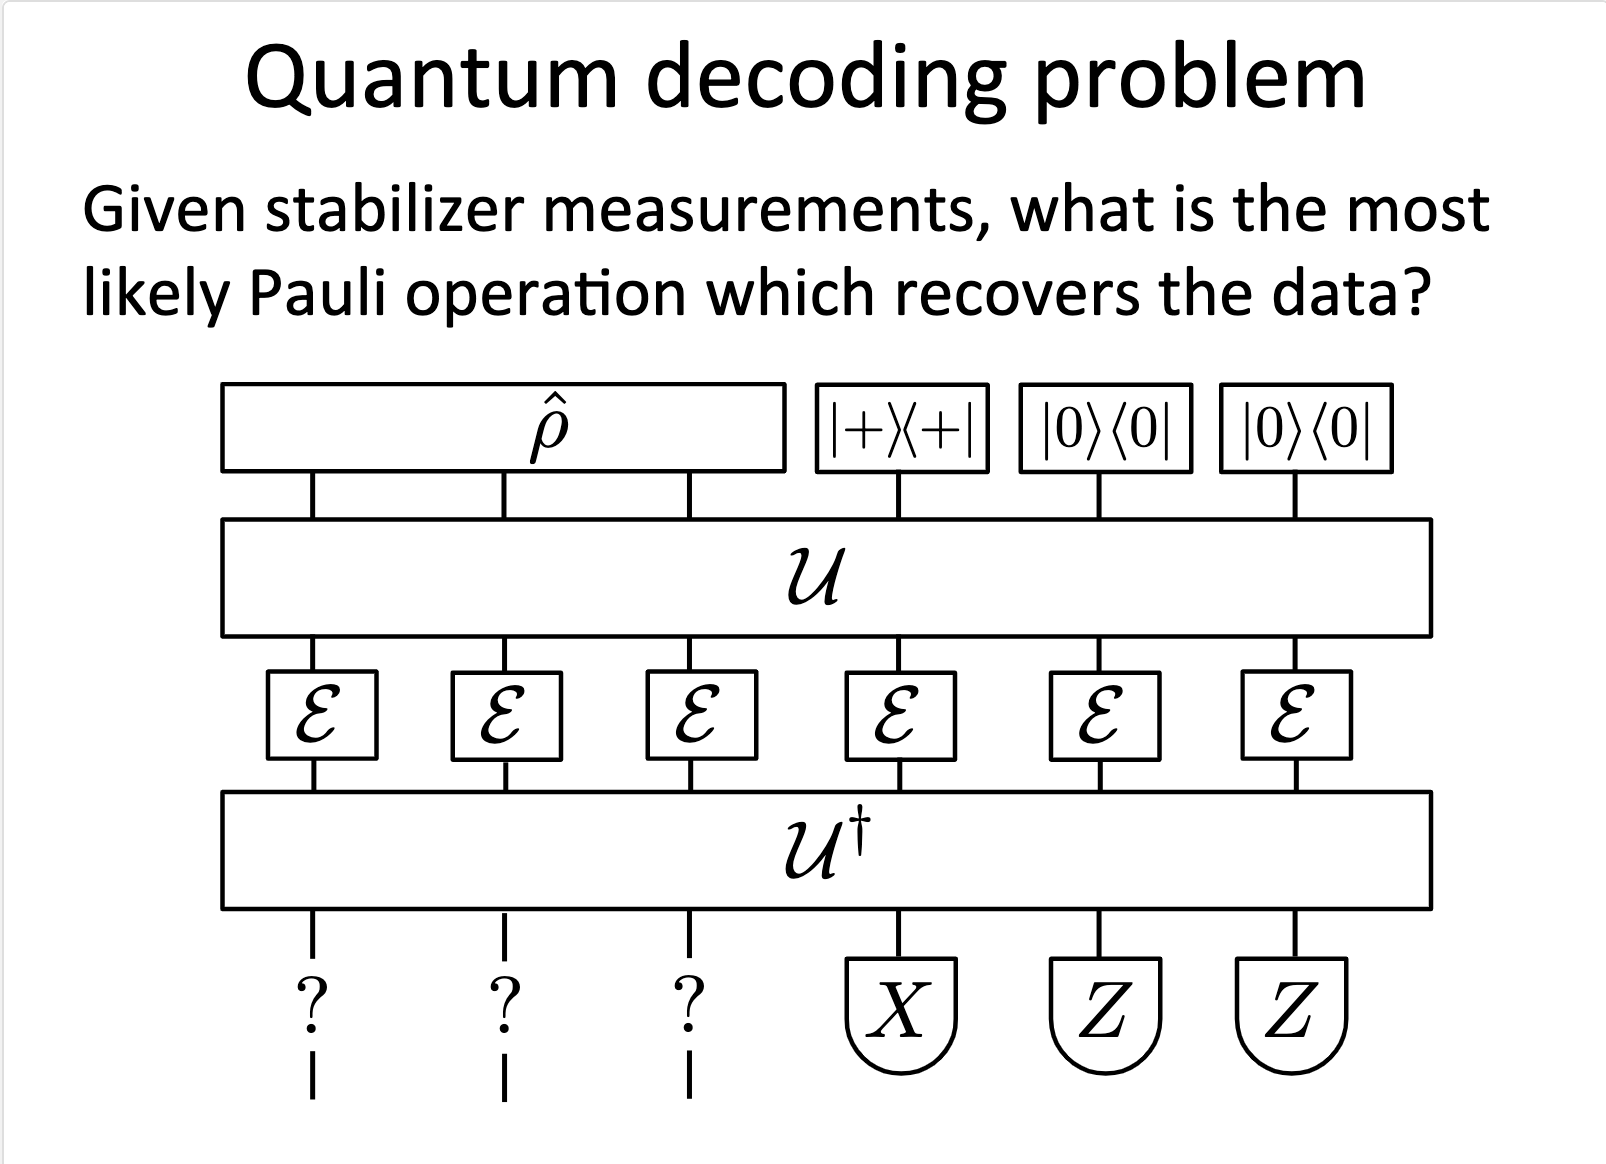
\includegraphics[scale=0.3]{../assets/decoding_gate_picture.png}
    \caption{Gate Picture of the Decoding problem. \textcolor{BrickRed}{What are the stabilizers in this picture?}}
    \label{fig:decode-gate-picture}
\end{figure}

In Fig. \ref{fig:decode-gate-picture}, you have tensor networks picture of the following process described in the equation below.
\begin{equation*}
    \rho \rightarrow Encode \rightarrow Error \rightarrow De-Encode \rightarrow Measure/Decode
\end{equation*}

\begin{figure}[ht]
    \centering
    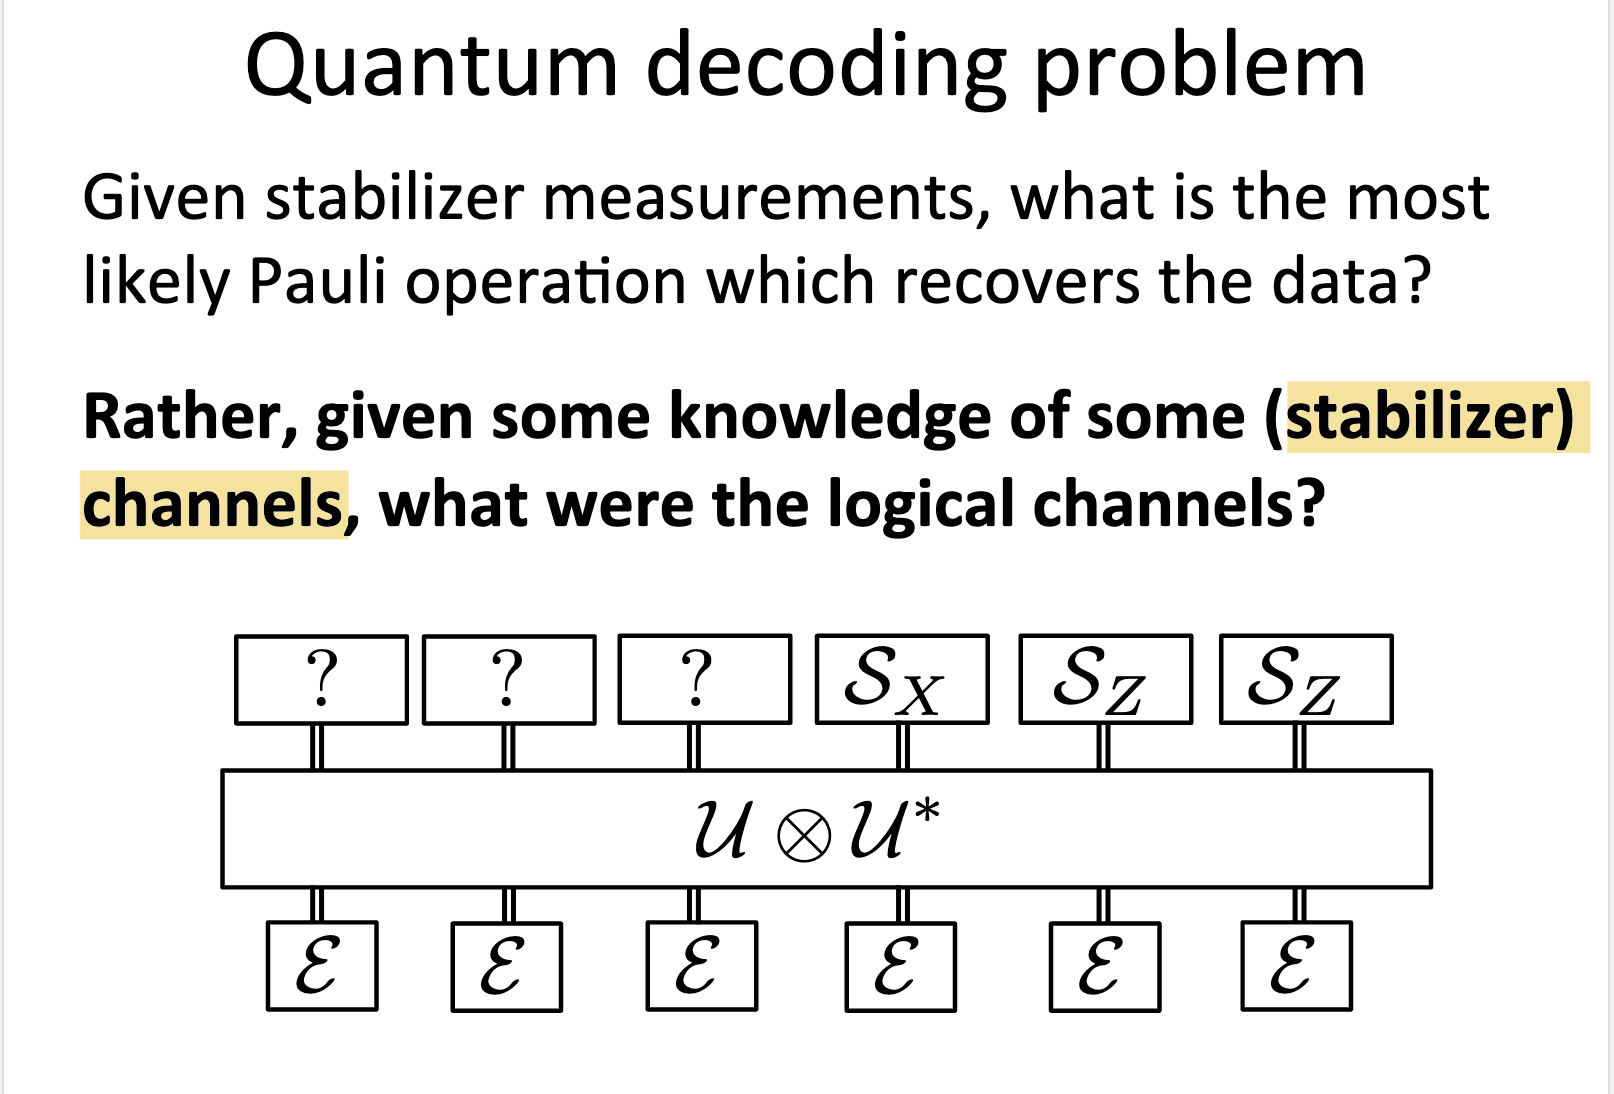
\includegraphics[scale=0.3]{../assets/decoding_channel_picture.png}
    \caption{Channel Picture of the Decoding problem. \textcolor{BrickRed}{What are the stabilizers in this picture?}}
    \label{fig:decode-channel-picture}
\end{figure}


\begin{quote}
    Thoughts from Alex Müller Hermes. For the Pauli Channel picture, Poulin is probably using one of the following. 
    \begin{align*}
        \rho \rightarrow \sum_{i = {0,1 2,3}} p_i Tr(\sigma_i \rho) \\
        \rho \rightarrow \sum_{i = {0,1 2,3}} p_i  \sigma_i \rho \sigma_i  \\
    \end{align*}
    In the end, this makes sense, because he is just re-orderding the tensor network in a different way. He did say something along the lines of prepare and measure $\ket{0}$.
\end{quote}

\textbf{How does $e = (1,1,1,1)$ correspond to the partial trace operations?}
\begin{itemize}
    \item If I just do it for single qubit line, it should correspond to the trace operation. Maybe this condition does not make sense.(Why?)
    \item If I do it for a bell pair, the partical trace should give me a maximally mixed state.
\end{itemize}

How to write the partial trace operation in the operator basis. What you get out in the end is the coefficient for the matrices $\{I, X, Y, Z\}$
Doing it in a single qubit line, given a state, in the form a density matrix $\rho$. Is there a requirment to choose a basis when performing the trace?

\begin{align*}
    \text{Trace} \equiv 
\end{align*}

Say I have single qubit density matrix $\rho$, which is a $rank-2$ tensor. What does $Tr(\sigma_j \rho)$ give me? It gives the expectation value of the measurement along the $\sigma_j$ axis of the qubit. Since ${\sigma_j}$ form a basis for the operator space of single qubit operations, any single qubit transformation can be characterized by 


\textbf{How does $b_z =(1,0,0,1)$ and $\bar{b_z} = (0,1,1,0)$ correspond to syndromes 0 and 1 respectively?}
One construct $b_z$ by the measure and prepare hypothesis. This being, if you prepare it in one of the eigenstate of the measurement basis, then it stays in the same eigenstate when there is no error. The nomenclature Quantum Stabilizer Channels makes no sense as it's a misnomer and can lead to the reader thinking this channel auto reverts from the onset of an error to one of the stabilizer states. 



\section{On indicator functions}
In appendix A of DP 2017, the author provide a presricption for representing a channel using a $4 \times 4$ process matrix. This section tries to reason how one may arrive at the indicator functions taking advantage of the channel-state duality offered by the Choi-Jamiolkowski Isomorphism. Ferris, in his talk on Tensor Networks and Quantum Error Correction, reposed the decoding channel in terms of channels. In partcular, he has asks: Given knowledge of some stabilizer channels, what the logical channel of the data qubits or the logical channel of the logical qubits. Poulin's reuses this framework in Tensor Networks Simulations of the Surface Code, in his 2017 paper Darmawan. 


Biamonte in his lectures on Quantum Tensor Networks, shows how to model the Choi Jamilowski Isomorphism as Tensor Network, adding an extra index for each qubit. 

\end{document}